\documentclass[10pt,a4paper]{amsart}
\usepackage[margin=19mm]{geometry}
\usepackage{amsmath,amssymb,mathtools}
\usepackage[scr=rsfs,cal=euler]{mathalfa}
\usepackage{xfrac}
\usepackage[unicode,hidelinks,bookmarks=false]{hyperref}
\newcommand{\ie}{i.e.\ }
\newcommand{\cf}{cf.\ }
\newcommand{\resp}{respectively\ }
\newcommand{\Subsection}{\subsection}
\providecommand{\nobreakdash}{\nobreak\hbox{-}}
\setlength{\emergencystretch}{2em}
\multlinegap0pt
\usepackage{tikz}
\usepackage{amssymb}
\usepackage{bm}
\usepackage{mathtools}
\usepackage{braket}
\usepackage[shortlabels]{enumitem}
\usepackage{tcolorbox}
\newtheorem{definizione}{Definition}
\newtheorem{lemma}{Lemma}
\newcommand{\OO}{\text{\normalfont  O}}
\DeclareMathOperator{\R}{\mathbb{R}}
\newcommand{\abs}[1]{{\left|#1\right|}}
\title{On the stability of the annulus for the torsion of multiply connected domains}
\author{Vincenzo Amato, Luca Barbato}
\date{Source: arXiv:2506.07592v2 (CC BY 4.0)}
\begin{document}
\maketitle

\noindent\emph{Source and licence.} On the stability of the annulus for the torsion of multiply connected domains. Version arXiv:2506.07592v2 (CC BY 4.0), distributed by arXiv under the Creative Commons Attribution 4.0 International licence, http://creativecommons.org/licenses/by/4.0/, as recorded in the arXiv licence metadata for this exact version and shown on the abstract page https://arxiv.org/abs/2506.07592v2. Full licence notice: \texttt{licenses/arxiv-2506.07592-CC-BY-4.0.txt}.\par\smallskip

\noindent\textit{Editorial scope.} Counted unit: the article's lemma lemma5.2 (source0.tex lines 929--936). The article's complete original proof of it is delivered with it (source0.tex lines 1076--1227, one \texttt{proof} environment of 152 lines, which the article places away from the statement). No mathematics is written, repaired or re-derived: the statement and the proof are the article's own lines, in the article's own notation, and no retained line is substituted or re-flowed.  Retained uncounted as the source-local context the proof needs: lines 119--128; lines 1017--1020.  Nothing was omitted from any retained span, so the package carries no omission record.  No retained line contains a citation, so the wrapper carries no bibliography and no bibliography entry.  The retained lines contain the article's own diagram code, which the wrapper typesets with the standard tikz packages; no image file is delivered and the package declares no asset dependency.  Editorial formatting only, in addition: an AMS \texttt{amsart} preamble that restates the article's own declarations and macros used by the retained lines, namely the environments \texttt{definizione}, \texttt{lemma} on separate counters, together with the standard packages those lines need.  The retained environments print in this document as Definizione 1, Lemma 1 in order of appearance, whereas the article prints the same items with the numbering of its own full document.  The complete native source of the article as distributed in the arXiv e-print for this exact version is bundled unchanged as \texttt{sources/179542/source0.tex}.
\begin{definizione}
    \label{multiplyconnected}
    A set $\Omega$ is a multiply connected domain if  $\Omega=G\setminus S$ and the following properties hold:
\begin{itemize}
    \item[\emph{(i)}] there exist $G,\Omega_1,\dots,\Omega_m$ bounded Lipschitz domain of $\R^n$; 
    \item[\emph{(ii)}] $\overline{\Omega}_i\subset G$ for $i=1,\dots,m$;
    \item[\emph{(iii)}]$\overline{\Omega}_i\cap\overline{\Omega}_j=\emptyset$ if $i\neq j$;
    \item[\emph{(iv)}]$S=\bigcup\limits_{i=1}^m\overline{\Omega}_i$.    
\end{itemize}
\end{definizione}

    \begin{equation}
        \label{essastorsion}
         T(\Omega^\OO)- T(\Omega)\geq  (u^\ast\left(\abs{S}\right) -s_{\tilde{S}})\abs{S}\frac{\alpha(\tilde{ S})^2}{9\gamma_n},
    \end{equation}

\begin{lemma}\label{lemma5.2}
	Let $\Omega\subset\R^2$ satisfy Definition \ref{multiplyconnected}. Let $\tilde{S}=D_{\tilde u}(\abs{S})$, if
    \[\abs{S}\leq\frac{2}{3}\abs{G}.\]
    Then 
    \begin{equation*}
    T(\Omega^\OO)-T(\Omega) \geq \frac{\abs{S}^2\alpha(\tilde{S})^3}{3^22^4\pi \gamma_ 2}.
\end{equation*}
\end{lemma}

\begin{proof}[Proof of Lemma \ref{lemma5.2}]
    We define $t_1$ such that
    \begin{equation*}
        \mu_{\tilde V}(\tilde V(\abs{S})-2t_1)=\abs{S}\left(1+\frac{1}{4}\alpha(\tilde{S})\right).
    \end{equation*}

        By $\abs{S} \leq \frac{2}{3}\abs{G}$, we have $ \mu_{\tilde V}(\tilde V(\abs{S})-2t_1) \leq \abs{G}$. Therefore,  the following  holds
    \begin{equation*}
        \begin{aligned}
            \frac{\abs{S}\alpha(\tilde{S})}{4}=\abs{S}\left(1+\frac{1}{4}\alpha(\tilde{S})\right)-\abs{S}=\mu_{\tilde V}(\tilde V(\abs{S})-2t_1)-\mu_{\tilde V}(\tilde V(\abs{S}))=\\-\int_{V(\abs{S})-2t_1}^{V(\abs{S})}\mu_{\tilde V}'(s)\,ds=4\pi\int_{V(\abs{S})-2t_1}^{V(\abs{S})}\,ds=8\pi t_1,
        \end{aligned}
    \end{equation*}
 where the last equality follows from symmetry. Indeed, since $\tilde V$ is radial, its superlevel sets are balls. Hence
\begin{equation*}
P(\tilde V>t)^2 = 4\pi\,\mu_{\tilde V}(t).
\end{equation*}
Moreover, for every $t \in (0, V(|S|))$ we have
\begin{equation*}
\begin{aligned}
P(\tilde V>t)^2
&=\left(-\frac{d}{dt}\int_t^\infty P(\tilde V>s)\,ds\right)^2 \\
&=\left(-\frac{d}{dt}\int_{\{\tilde V>t\}}|\nabla V|\,dx\right)^2 \\
&=\left(-\frac{d}{dt}\int_{\{\tilde V>t\}} \,dx\right)
  \left(-\frac{d}{dt}\int_{\{\tilde V>t\}} |\nabla V|^2\,dx\right) \\
&= -\mu_{\tilde V}'(t)\,\mu_{\tilde V}(t),
\end{aligned}
\end{equation*}
where in the last step we used the coarea formula.

Combining the two identities, we have
\[
-\mu_{\tilde V}'(t)\,\mu_{\tilde V}(t) = 4\pi\,\mu_{\tilde V}(t),
\]
and therefore, for every $t$ such that $\mu_{\tilde V}(t)>0$,
\begin{equation}\label{muprimo=4pi}
-\mu_{\tilde V}'(t) = 4\pi.
\end{equation} 
     Also the pointwise comparison gave us a bound on $s_{\tilde{S}}$ as
    \begin{equation}\label{boundss}
        \tilde V(\abs{S})-2t_1=\tilde V\left(\abs{S}\left(1+\frac{1}{4}\alpha(\tilde{S})\right)\right)\geq\tilde u^\ast\left(\abs{S}\left(1+\frac{1}{4}\alpha(\tilde{S})\right)\right)=s_{\tilde{S}}.
    \end{equation}
    Now let us distinguish two cases:
    \begin{itemize}
        \item if $\tilde V(\abs{S})-\tilde u^\ast(\abs{S})<t_1$, then from \eqref{essastorsion} and \eqref{boundss}\, we obtain
        \begin{equation*}
            {\tilde u}^\ast(\abs{S})-s_{\tilde{S}}\geq\tilde u^\ast(\abs{S})-\tilde V(\abs{S})+2t_1\geq -t_1+2t_1=\frac{\abs{S}\alpha(\tilde{S})}{2^5\pi},
         \end{equation*}
        hence, we have

         \begin{equation*}
              T(\Omega^\OO)-T(\Omega)\geq   (u^\ast\left(\abs{S}\right) -s_{\tilde{S}})\abs{S}\frac{2\alpha({\tilde{S}})^2}{9\gamma_n} \geq \frac{\abs{S}^2\alpha(\tilde{S})^3}{3^22^4\pi \gamma_ 2}.
         \end{equation*}


         \item if $\tilde V(\abs{S})-\tilde u^\ast(\abs{S})\geq t_1$, we define the function \begin{equation*}%\label{funzionefbound}
          f(s)=
         \begin{cases}
         \tilde V (\abs{S}) & \text{ if } s \leq \abs{S}\\
             u^\ast (\abs{S})& \text{ if }  \abs{S} < s \leq \abs{S} + 4\pi \left(\tilde V(\abs{S})-\tilde u^\ast(\abs{S})\right) \\
              \tilde V(s)& \text{ if }  \abs{S} + 4 \pi \left(\tilde V(\abs{S})-\tilde u^\ast(\abs{S})\right)   <s \leq \abs{G},
         \end{cases}\end{equation*}
         
         which is greater or equal to $\tilde u^\ast$ (see figure \ref{fig:funzionef}).
         
         Hence, we have 
         \begin{equation}
             \label{claimbho}
             \begin{aligned}
                 T(\Omega^\OO)-T(\Omega)&=\int _0^{\abs{G}} \left(\tilde V(s)-\tilde u^\ast(s)\right)\, ds \\
                 &\geq \int _0^{\abs{G}} \left(\tilde V(s)-f(s)\right)\, ds= 2 \pi \left(\tilde V(\abs{S})-\tilde u^\ast(\abs{S})\right)^2.
             \end{aligned}
             \end{equation} 

             The latter, after some computations,  gives
              \begin{equation*}
             T(\Omega^\OO)-T(\Omega)\geq 2 \pi \left(\tilde V(\abs{S})-\tilde u^\ast(\abs{S})\right)^2\geq 2 \pi t_1^2\geq \frac{2 \pi}{2^{10} \pi^2}\abs{S}^2\alpha(\tilde{S})^2\geq \frac{\abs{S}^2\alpha(\tilde{S})^3}{2^{10} \pi}.
         \end{equation*}
         
         
    \end{itemize}
      \begin{figure}[ht!]
        \centering
        


\tikzset{every picture/.style={line width=0.75pt}} %set default line width to 0.75pt        

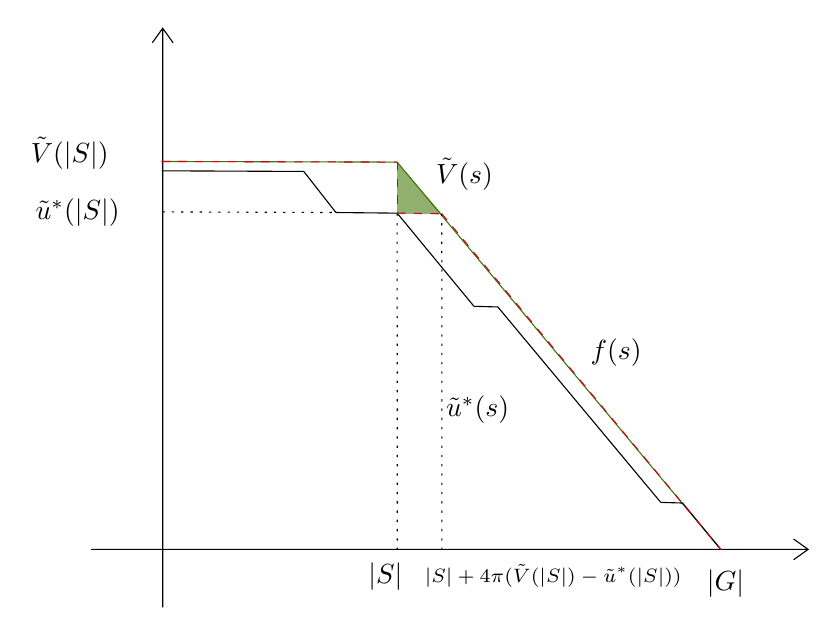
\begin{tikzpicture}[x=0.75pt,y=0.75pt,yscale=-1,xscale=1]
%uncomment if require: \path (0,300); %set diagram left start at 0, and has height of 300

%Straight Lines [id:da5594649633021156] 
\draw  [dash pattern={on 0.84pt off 2.51pt}]  (292.5,104.7) -- (292.55,266.32) ;
%Straight Lines [id:da5942426507868859] 
\draw [color={rgb, 255:red, 0; green, 0; blue, 0 }  ,draw opacity=1 ] [dash pattern={on 0.84pt off 2.51pt}]  (179.5,103.78) -- (188.75,103.82) -- (263,104.09) ;
%Shape: Right Triangle [id:dp26763058469178014] 
\draw  [draw opacity=0][fill={rgb, 255:red, 65; green, 117; blue, 5 }  ,fill opacity=0.58 ] (292.5,79.8) -- (314,104.7) -- (292.5,104.7) -- cycle ;
%Shape: Axis 2D [id:dp7032668208380202] 
\draw  (145,266.4) -- (490.5,266.4)(179.55,15.3) -- (179.55,294.3) (483.5,261.4) -- (490.5,266.4) -- (483.5,271.4) (174.55,22.3) -- (179.55,15.3) -- (184.55,22.3)  ;
%Straight Lines [id:da2947591129314542] 
\draw [color={rgb, 255:red, 65; green, 117; blue, 5 }  ,draw opacity=1 ]   (179,79.5) -- (292.5,79.8) ;
%Straight Lines [id:da15806518879650078] 
\draw [color={rgb, 255:red, 65; green, 117; blue, 5 }  ,draw opacity=1 ]   (292.5,79.8) -- (448.5,266.5) ;
%Straight Lines [id:da5484709852409027] 
\draw [color={rgb, 255:red, 0; green, 0; blue, 0 }  ,draw opacity=1 ]   (179,84) -- (247.5,84.3) ;
%Straight Lines [id:da5662895113598212] 
\draw [color={rgb, 255:red, 0; green, 0; blue, 0 }  ,draw opacity=1 ]   (247.5,84.3) -- (263,104.09) ;
%Straight Lines [id:da5011809630795425] 
\draw    (292.5,104.39) -- (311,126.84) ;
%Straight Lines [id:da8674515481041667] 
\draw [color={rgb, 255:red, 0; green, 0; blue, 0 }  ,draw opacity=1 ]   (311,126.84) -- (329.5,149.28) ;
%Straight Lines [id:da8089452956814356] 
\draw    (430,244.05) -- (448.5,266.5) ;
%Straight Lines [id:da6572568937742018] 
\draw [color={rgb, 255:red, 0; green, 0; blue, 0 }  ,draw opacity=1 ]   (341,149.59) -- (419.5,243.75) ;
%Straight Lines [id:da8066824427181756] 
\draw [color={rgb, 255:red, 0; green, 0; blue, 0 }  ,draw opacity=1 ]   (419.5,243.75) -- (430,244.05) ;
%Straight Lines [id:da6010325590490861] 
\draw [color={rgb, 255:red, 0; green, 0; blue, 0 }  ,draw opacity=1 ]   (329.5,149.28) -- (341,149.59) ;
%Straight Lines [id:da9339825758405371] 
\draw [color={rgb, 255:red, 0; green, 0; blue, 0 }  ,draw opacity=1 ]   (263,104.09) -- (292.5,104.39) ;
%Straight Lines [id:da6689242214556868] 
\draw [dashed,color={rgb, 255:red, 208; green, 2; blue, 27 }  ,draw opacity=1 ]   (179,79.5) -- (292.5,79.8) ;
%Straight Lines [id:da9321419225717913] 
\draw [dashed,color={rgb, 255:red, 208; green, 2; blue, 27 }  ,draw opacity=1 ]   (292.5,104.39) -- (314,104.7) ;
%Straight Lines [id:da8425927555383188] 
\draw [dashed,color={rgb, 255:red, 208; green, 2; blue, 27 }  ,draw opacity=1 ]   (314,104.7) -- (448.5,266.5) ;
%Straight Lines [id:da5389907024655973] 
\draw [dashed,color={rgb, 255:red, 208; green, 2; blue, 27 }  ,draw opacity=1 ]   (292.5,79.8) -- (292.5,104.39) ;
%Straight Lines [id:da17883543304905292] 
\draw  [dash pattern={on 0.84pt off 2.51pt}]  (314,104.7) -- (314.05,266.32) ;

% Text Node
\draw (440.5,275.15) node [anchor=north west][inner sep=0.75pt]    {$\abs{G}$};
% Text Node
\draw (114.75,66.4) node [anchor=north west][inner sep=0.75pt]    {$\tilde V(\abs{S})$};
% Text Node
\draw (310,76.4) node [anchor=north west][inner sep=0.75pt]    {$\tilde V(s)$};
% Text Node
\draw (117,96.28) node [anchor=north west][inner sep=0.75pt]    {$\tilde u^\ast(\abs{S})$};
% Text Node
\draw (277.4,271.4) node [anchor=north west][inner sep=0.75pt]    {$\abs{S}$};
% Text Node
\draw (314.8,191.2) node [anchor=north west][inner sep=0.75pt]    {$\tilde u^\ast(s)$};
% Text Node
\draw (384.4,163.6) node [anchor=north west][inner sep=0.75pt]    {$f(s)$};
% Text Node
\draw (304.54,272.26) node [anchor=north west][inner sep=0.75pt]    {\scriptsize $\abs{S}+ 4 \pi (\tilde V(\abs{S})- \tilde u^\ast (\abs{S}))$};
\end{tikzpicture}
\caption{Upper bound for $\tilde u^\ast(s)$}
        \label{fig:funzionef}
    \end{figure}
\end{proof}

\end{document}
